\documentclass[]{article}
\usepackage{lmodern}
\usepackage{amssymb,amsmath}
\usepackage{ifxetex,ifluatex}
\usepackage{fixltx2e} % provides \textsubscript
\ifnum 0\ifxetex 1\fi\ifluatex 1\fi=0 % if pdftex
  \usepackage[T1]{fontenc}
  \usepackage[utf8]{inputenc}
\else % if luatex or xelatex
  \ifxetex
    \usepackage{mathspec}
  \else
    \usepackage{fontspec}
  \fi
  \defaultfontfeatures{Ligatures=TeX,Scale=MatchLowercase}
\fi
% use upquote if available, for straight quotes in verbatim environments
\IfFileExists{upquote.sty}{\usepackage{upquote}}{}
% use microtype if available
\IfFileExists{microtype.sty}{%
\usepackage{microtype}
\UseMicrotypeSet[protrusion]{basicmath} % disable protrusion for tt fonts
}{}
\usepackage[margin=1in]{geometry}
\usepackage{hyperref}
\hypersetup{unicode=true,
            pdftitle={Jackknife variance estimation corrections},
            pdfauthor={Xuelong Wang},
            pdfborder={0 0 0},
            breaklinks=true}
\urlstyle{same}  % don't use monospace font for urls
\usepackage{graphicx,grffile}
\makeatletter
\def\maxwidth{\ifdim\Gin@nat@width>\linewidth\linewidth\else\Gin@nat@width\fi}
\def\maxheight{\ifdim\Gin@nat@height>\textheight\textheight\else\Gin@nat@height\fi}
\makeatother
% Scale images if necessary, so that they will not overflow the page
% margins by default, and it is still possible to overwrite the defaults
% using explicit options in \includegraphics[width, height, ...]{}
\setkeys{Gin}{width=\maxwidth,height=\maxheight,keepaspectratio}
\IfFileExists{parskip.sty}{%
\usepackage{parskip}
}{% else
\setlength{\parindent}{0pt}
\setlength{\parskip}{6pt plus 2pt minus 1pt}
}
\setlength{\emergencystretch}{3em}  % prevent overfull lines
\providecommand{\tightlist}{%
  \setlength{\itemsep}{0pt}\setlength{\parskip}{0pt}}
\setcounter{secnumdepth}{5}
% Redefines (sub)paragraphs to behave more like sections
\ifx\paragraph\undefined\else
\let\oldparagraph\paragraph
\renewcommand{\paragraph}[1]{\oldparagraph{#1}\mbox{}}
\fi
\ifx\subparagraph\undefined\else
\let\oldsubparagraph\subparagraph
\renewcommand{\subparagraph}[1]{\oldsubparagraph{#1}\mbox{}}
\fi

%%% Use protect on footnotes to avoid problems with footnotes in titles
\let\rmarkdownfootnote\footnote%
\def\footnote{\protect\rmarkdownfootnote}

%%% Change title format to be more compact
\usepackage{titling}

% Create subtitle command for use in maketitle
\providecommand{\subtitle}[1]{
  \posttitle{
    \begin{center}\large#1\end{center}
    }
}

\setlength{\droptitle}{-2em}

  \title{Jackknife variance estimation corrections}
    \pretitle{\vspace{\droptitle}\centering\huge}
  \posttitle{\par}
    \author{Xuelong Wang}
    \preauthor{\centering\large\emph}
  \postauthor{\par}
      \predate{\centering\large\emph}
  \postdate{\par}
    \date{2019-11-08}

\usepackage{float,amsmath, bbm, siunitx, bm}
\usepackage{pdfpages}
\floatplacement{figure}{H}
\newcommand{\indep}{\rotatebox[origin=c]{90}{$\models$}}

\begin{document}
\maketitle

{
\setcounter{tocdepth}{2}
\tableofcontents
}
\section{Jackknife variance
correction}\label{jackknife-variance-correction}

If we assume the \(S\) is a smooth functions of emperical CDF,
especially a quadratic functions, then it can be shown the leading terms
of
\(E(\tilde{Var}(S(X_1, \dots, S_{n-1}))) \geq Var(S(X_1, \dots, S_{n-1}))\)
is a quadratic term in expecation. Therefore we could try to estimate
the quadratic term and correct the bias for the jackknife variance
estimation.

Define \(Q_{ii'} \equiv nS - (n-1)(S_{i} + S_{i'}) + (n-2)S_{(ii')}\),
then the correction will be \[
\hat{Var}^{corr}(S(X_1, \dots, X_n)) = \hat{Var}(S(X_1, \dots, X_n)) - \frac{1}{n(n-1)}\sum_{i < i'}(Q_{ii'}- \bar{Q})^2
\] where \(\bar{Q} = \sum_{i < i'}(Q_{ii'})/(n(n-1)/2)\)

\section{Simulation study compare two GCTA and
GCTA\_rr}\label{simulation-study-compare-two-gcta-and-gcta_rr}

GCTA\_rr is the \texttt{mixed.solve} function from \texttt{rrBLUP} r
package.\\
Based on the following simulation results,

\begin{enumerate}
\def\labelenumi{\arabic{enumi}.}
\tightlist
\item
  when \(n<p\) case, those two methods' results are very closed to each
  other.
\item
  when \(n>p\) case, in terms of effect estimation and jackknife
  variance estimation those two methods's reuslts are similar to each
  other. But for the variance corrections are quite different. That is
  the statistics \(Q\) of our method has a very large variance which
  leads to negative correction result.
\end{enumerate}

\subsubsection{setup}\label{setup}

\begin{itemize}
\tightlist
\item
  Independent
\item
  Normal
\item
  \(p = 100\)
\item
  \(n = \{50, 75,100, 150, 200\}\)
\item
  with interaction terms
\item
  main effect: \(Var(X^T\beta) = 8\) \newpage
\end{itemize}

\subsubsection{n = 50}\label{n-50}

\begin{verbatim}
        main_effect_GCTA v_jack v_jack_corr
GCTA                6.29    124       -92.6
GCTA_rr             6.29    124       -92.6
\end{verbatim}

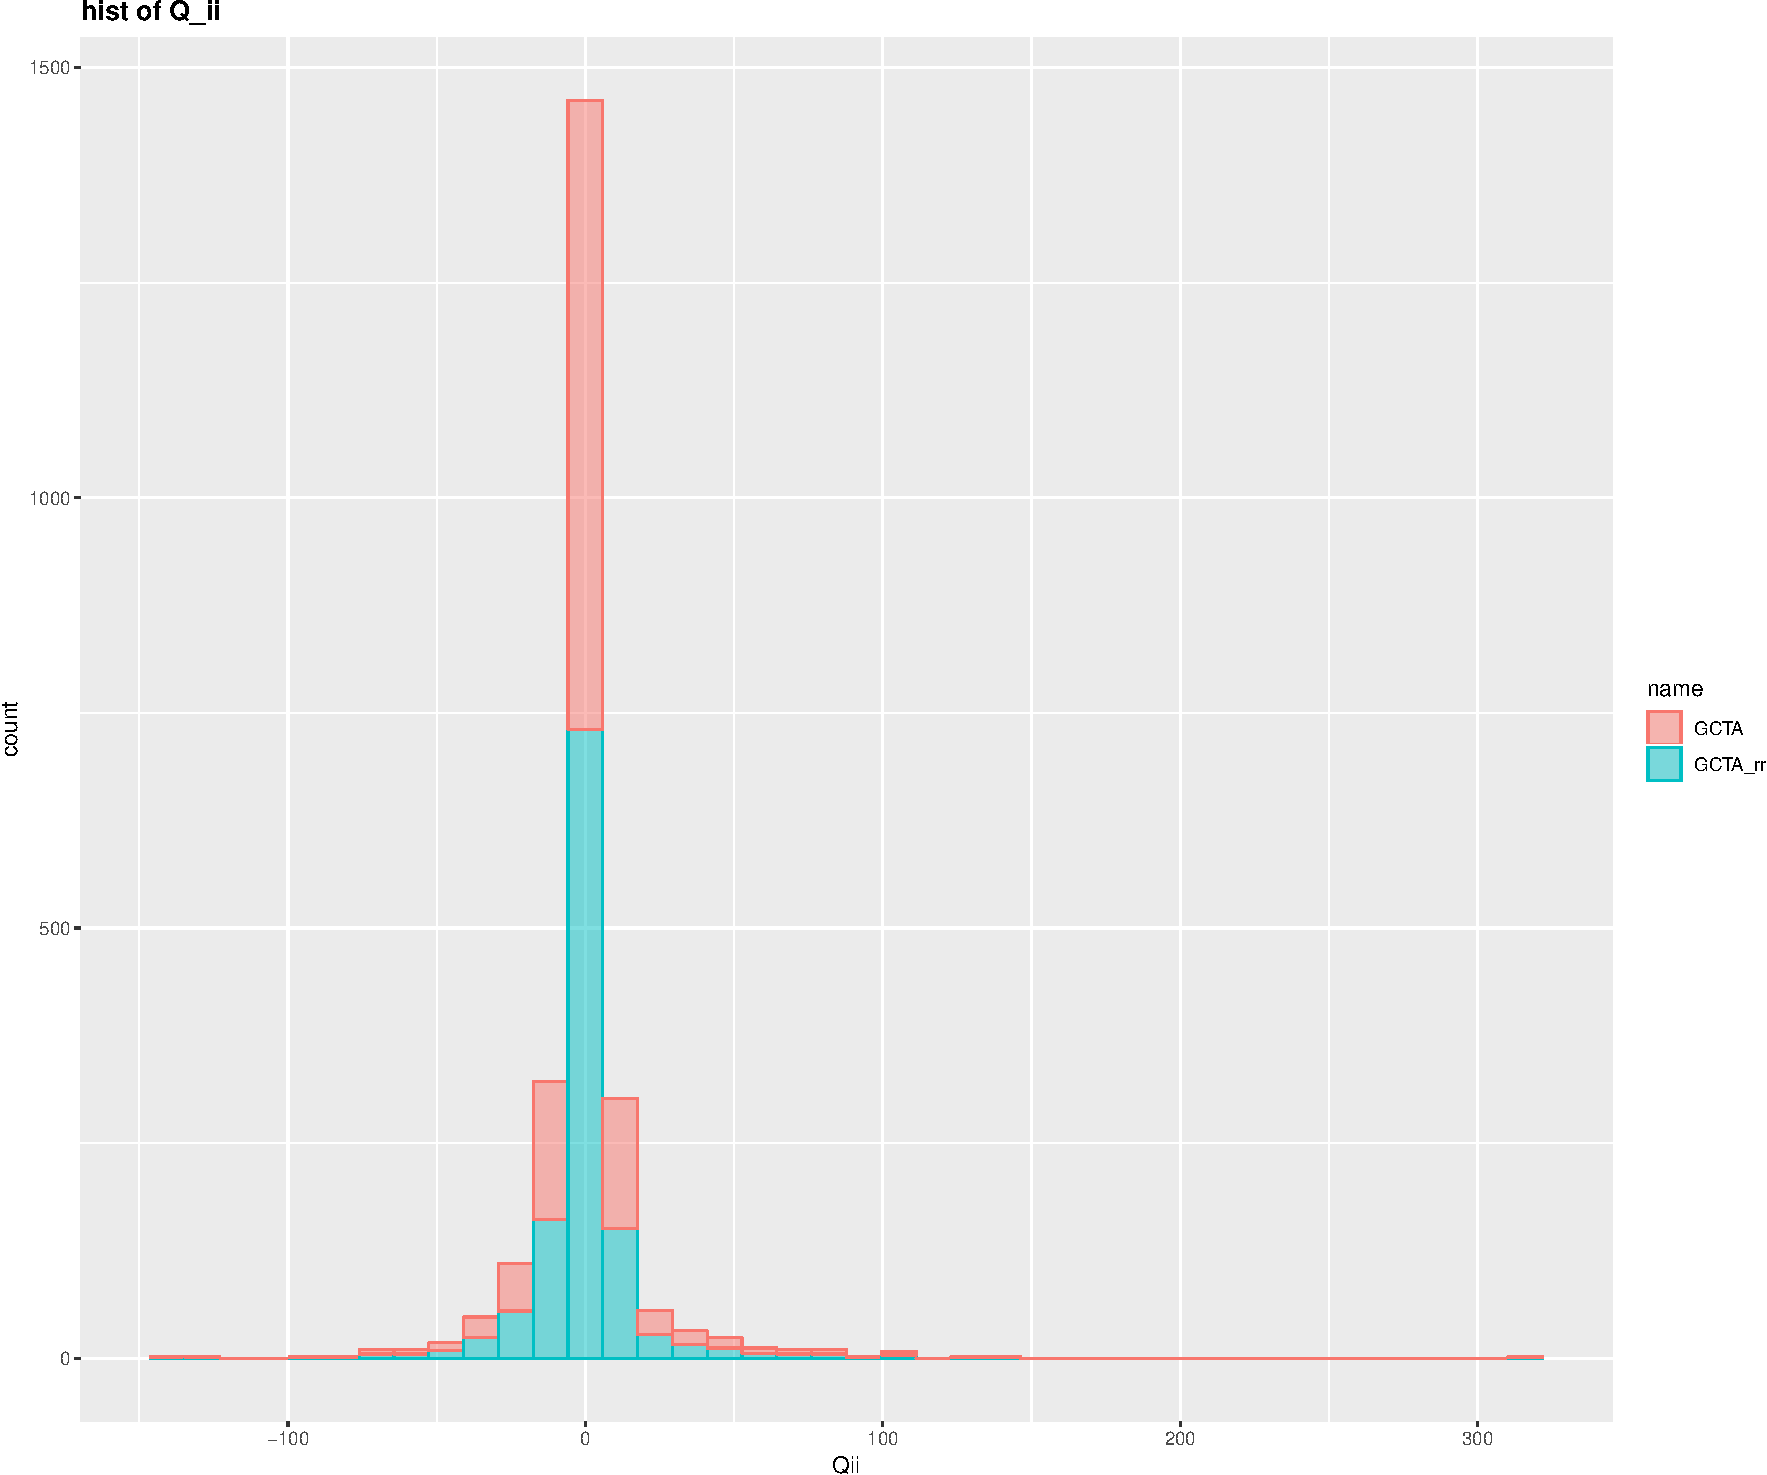
\includegraphics{GCTA_and_rr_v_jack_correction_files/figure-latex/unnamed-chunk-2-1.pdf}
\newpage

\subsubsection{n = 75}\label{n-75}

\begin{verbatim}
        main_effect_GCTA v_jack v_jack_corr
GCTA                 3.7     28        -9.4
GCTA_rr              3.7     28        -9.4
\end{verbatim}

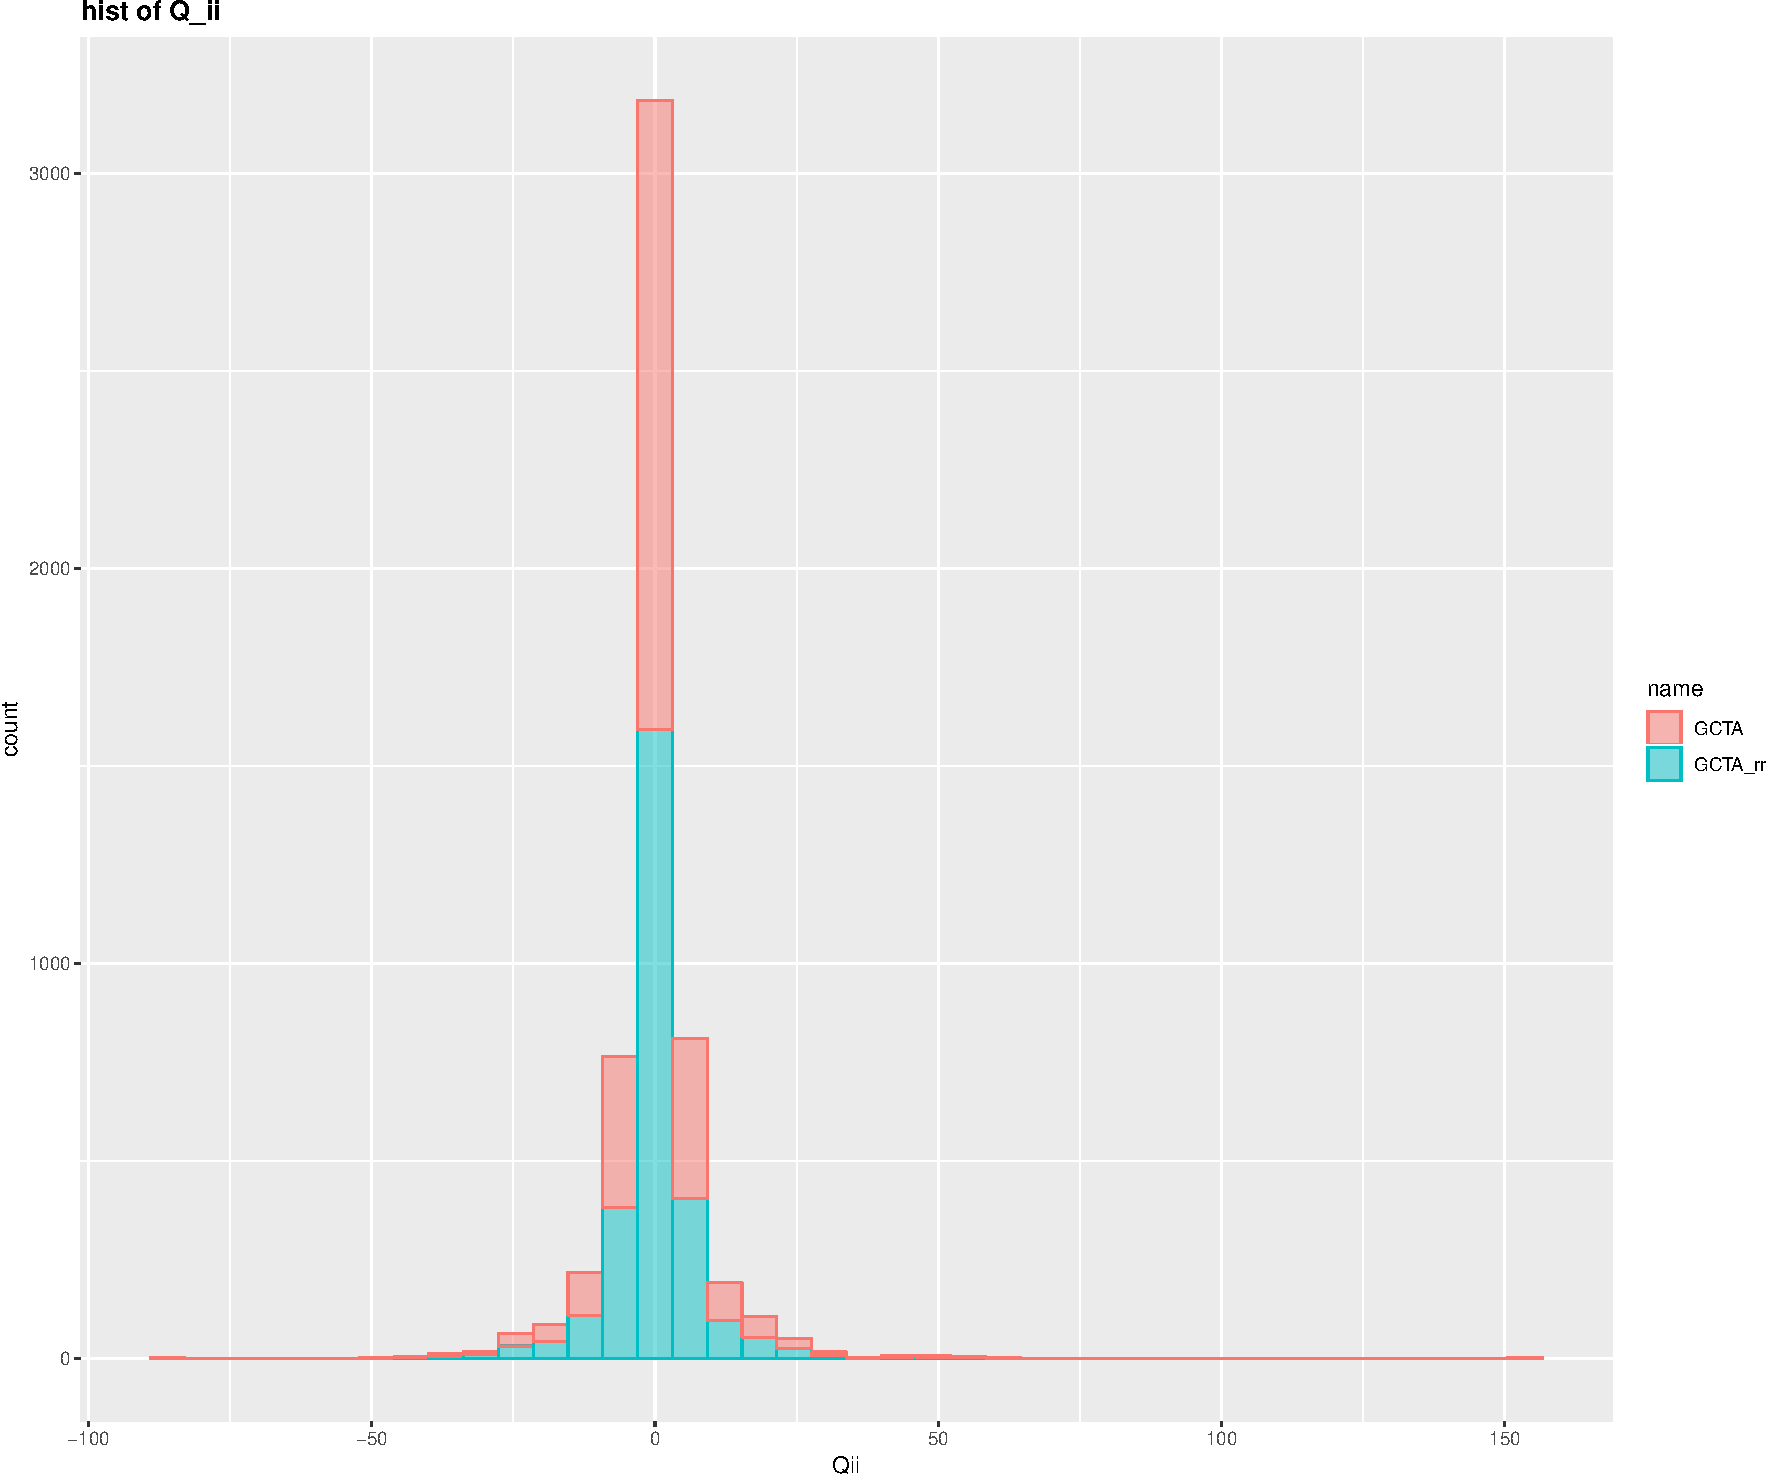
\includegraphics{GCTA_and_rr_v_jack_correction_files/figure-latex/unnamed-chunk-3-1.pdf}
\newpage

\subsubsection{n = 100}\label{n-100}

\begin{verbatim}
        main_effect_GCTA v_jack v_jack_corr
GCTA                8.41   9.68       -1.08
GCTA_rr             8.41   9.68       -1.08
\end{verbatim}

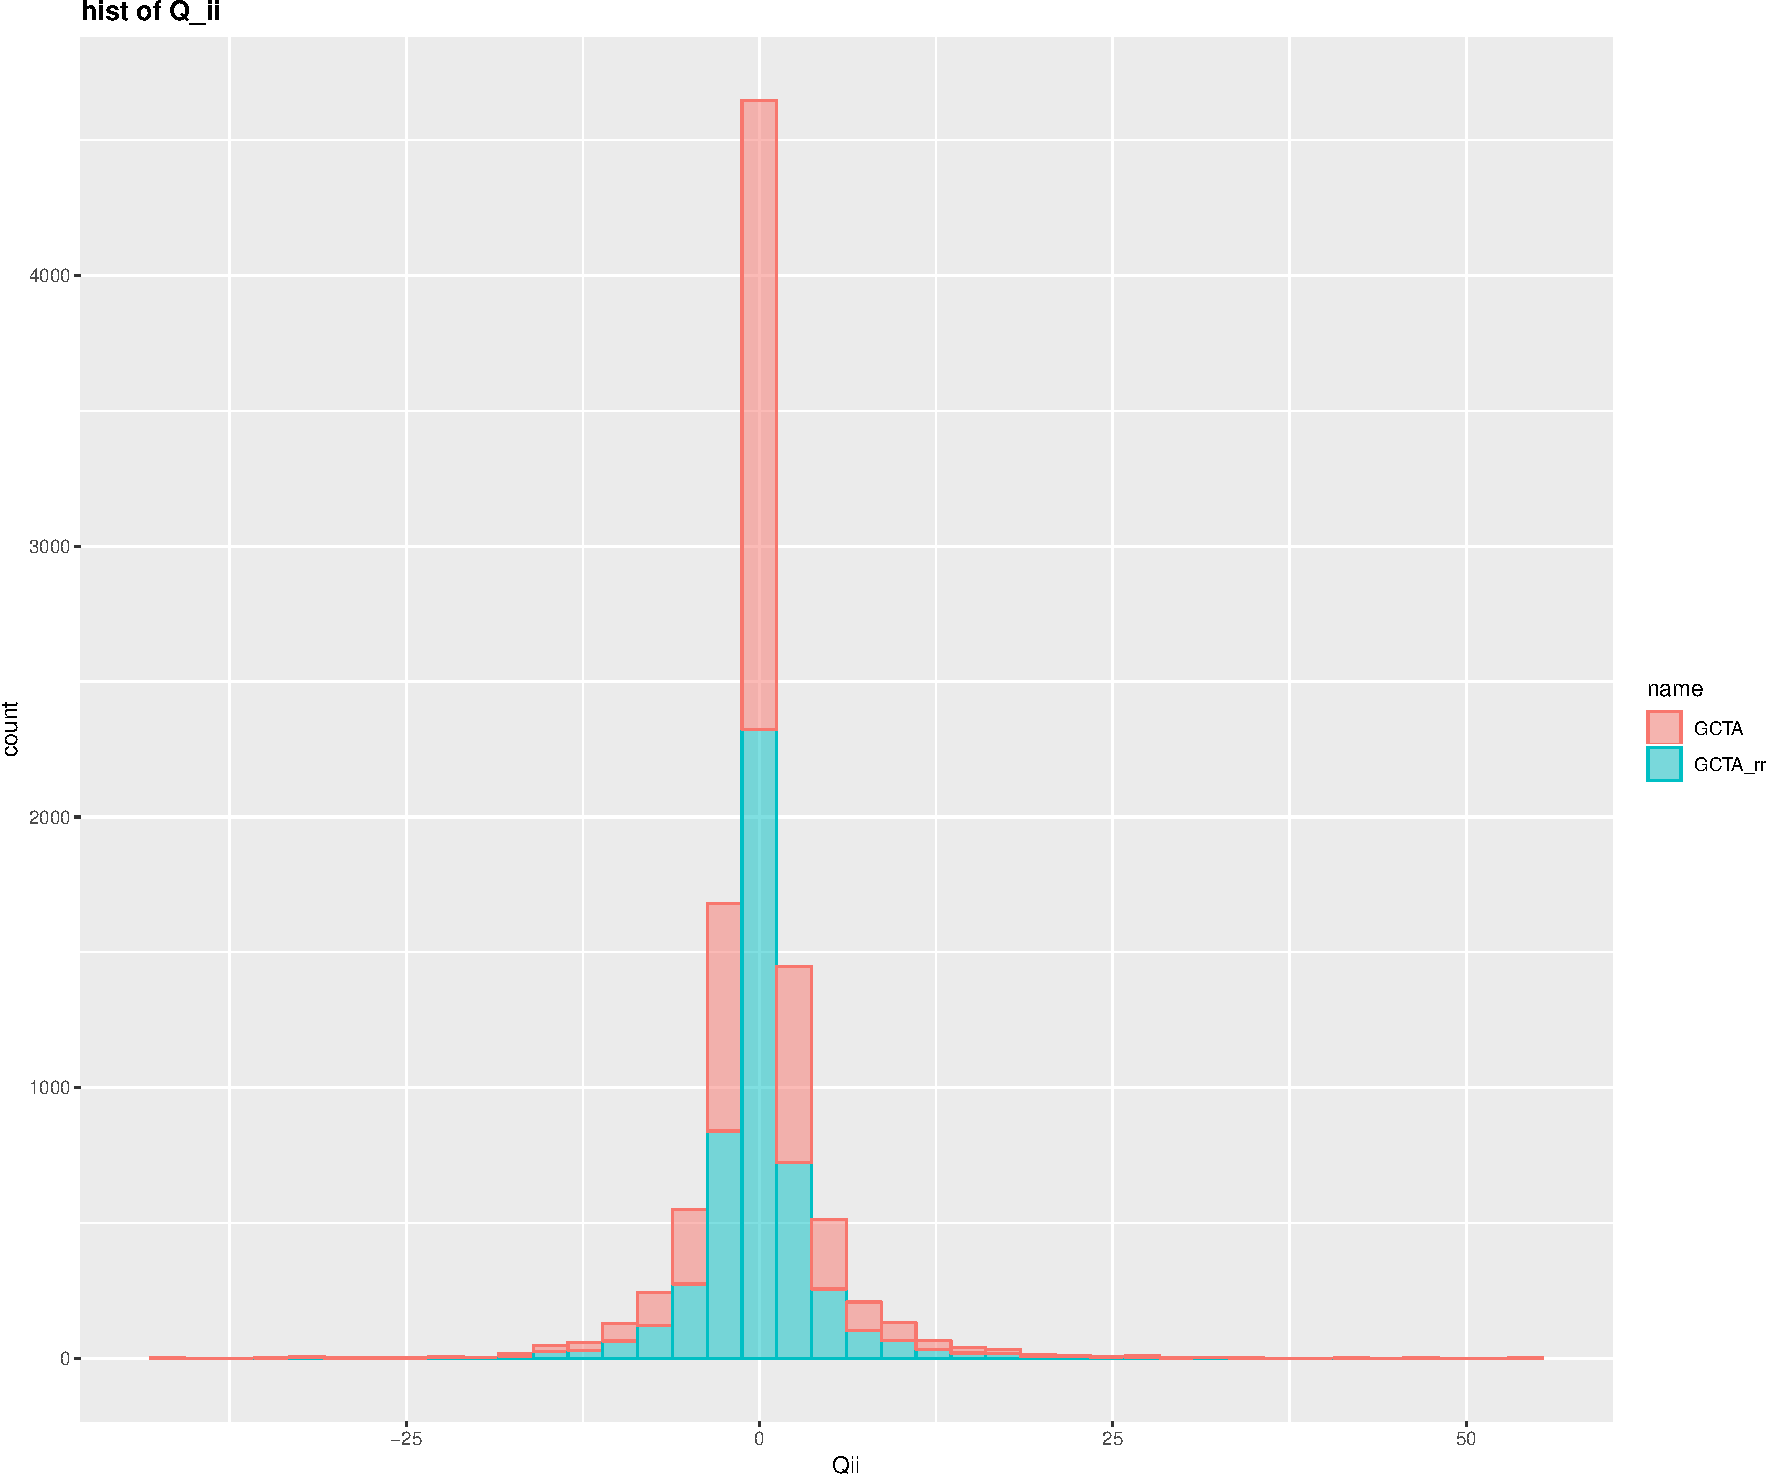
\includegraphics{GCTA_and_rr_v_jack_correction_files/figure-latex/unnamed-chunk-4-1.pdf}
\newpage

\subsubsection{n = 150}\label{n-150}

\begin{verbatim}
        main_effect_GCTA v_jack v_jack_corr
GCTA                8.47   8.73     -478.33
GCTA_rr             8.50   6.35        1.57
\end{verbatim}

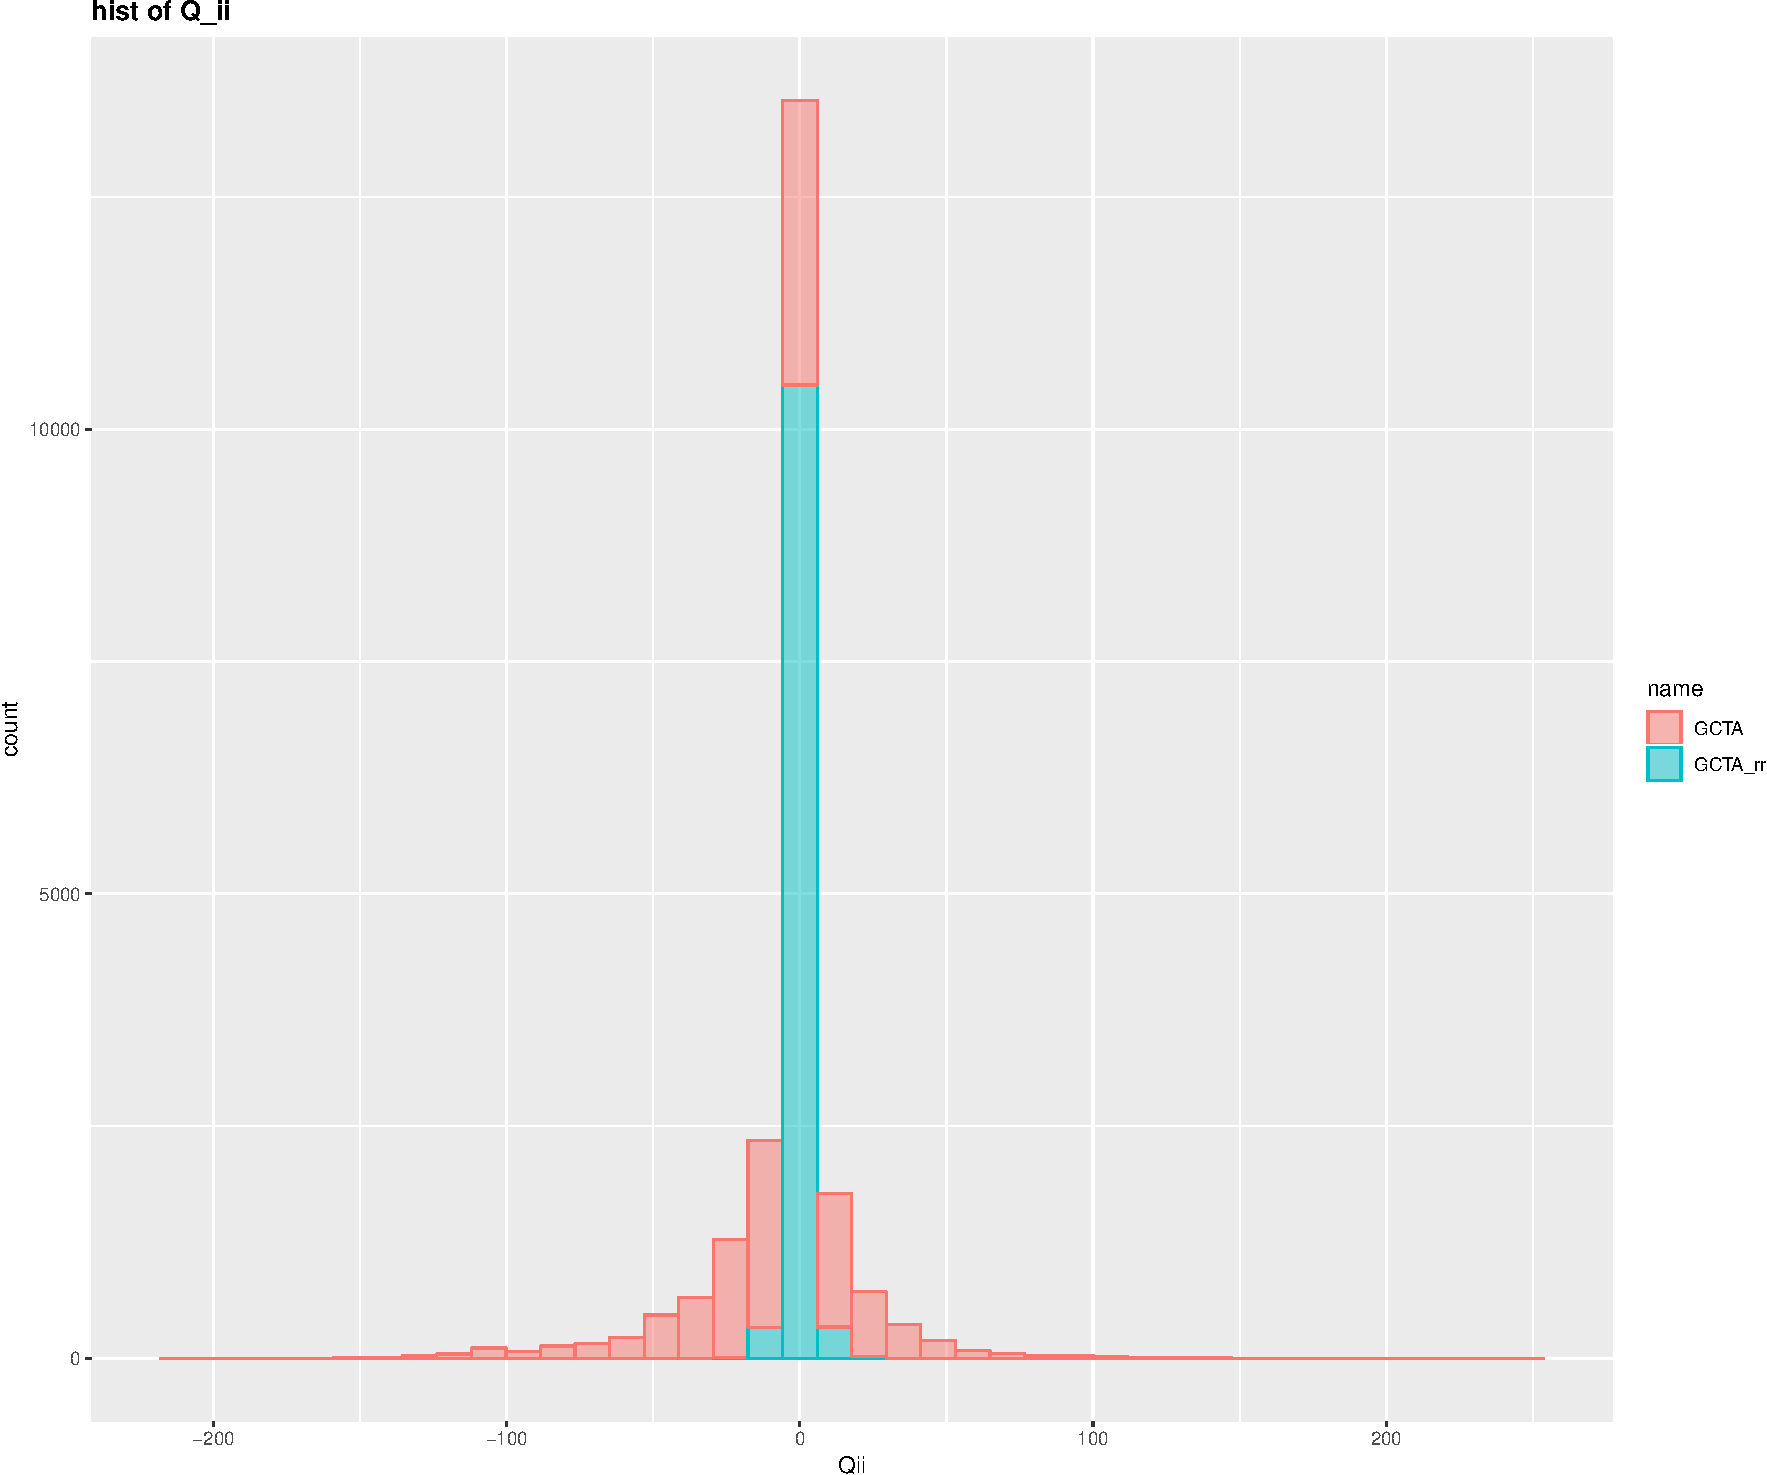
\includegraphics{GCTA_and_rr_v_jack_correction_files/figure-latex/unnamed-chunk-5-1.pdf}
\newpage

\subsubsection{n = 200}\label{n-200}

\begin{verbatim}
        main_effect_GCTA v_jack v_jack_corr
GCTA                8.56   3.96     -137.52
GCTA_rr             8.58   3.64        1.61
\end{verbatim}

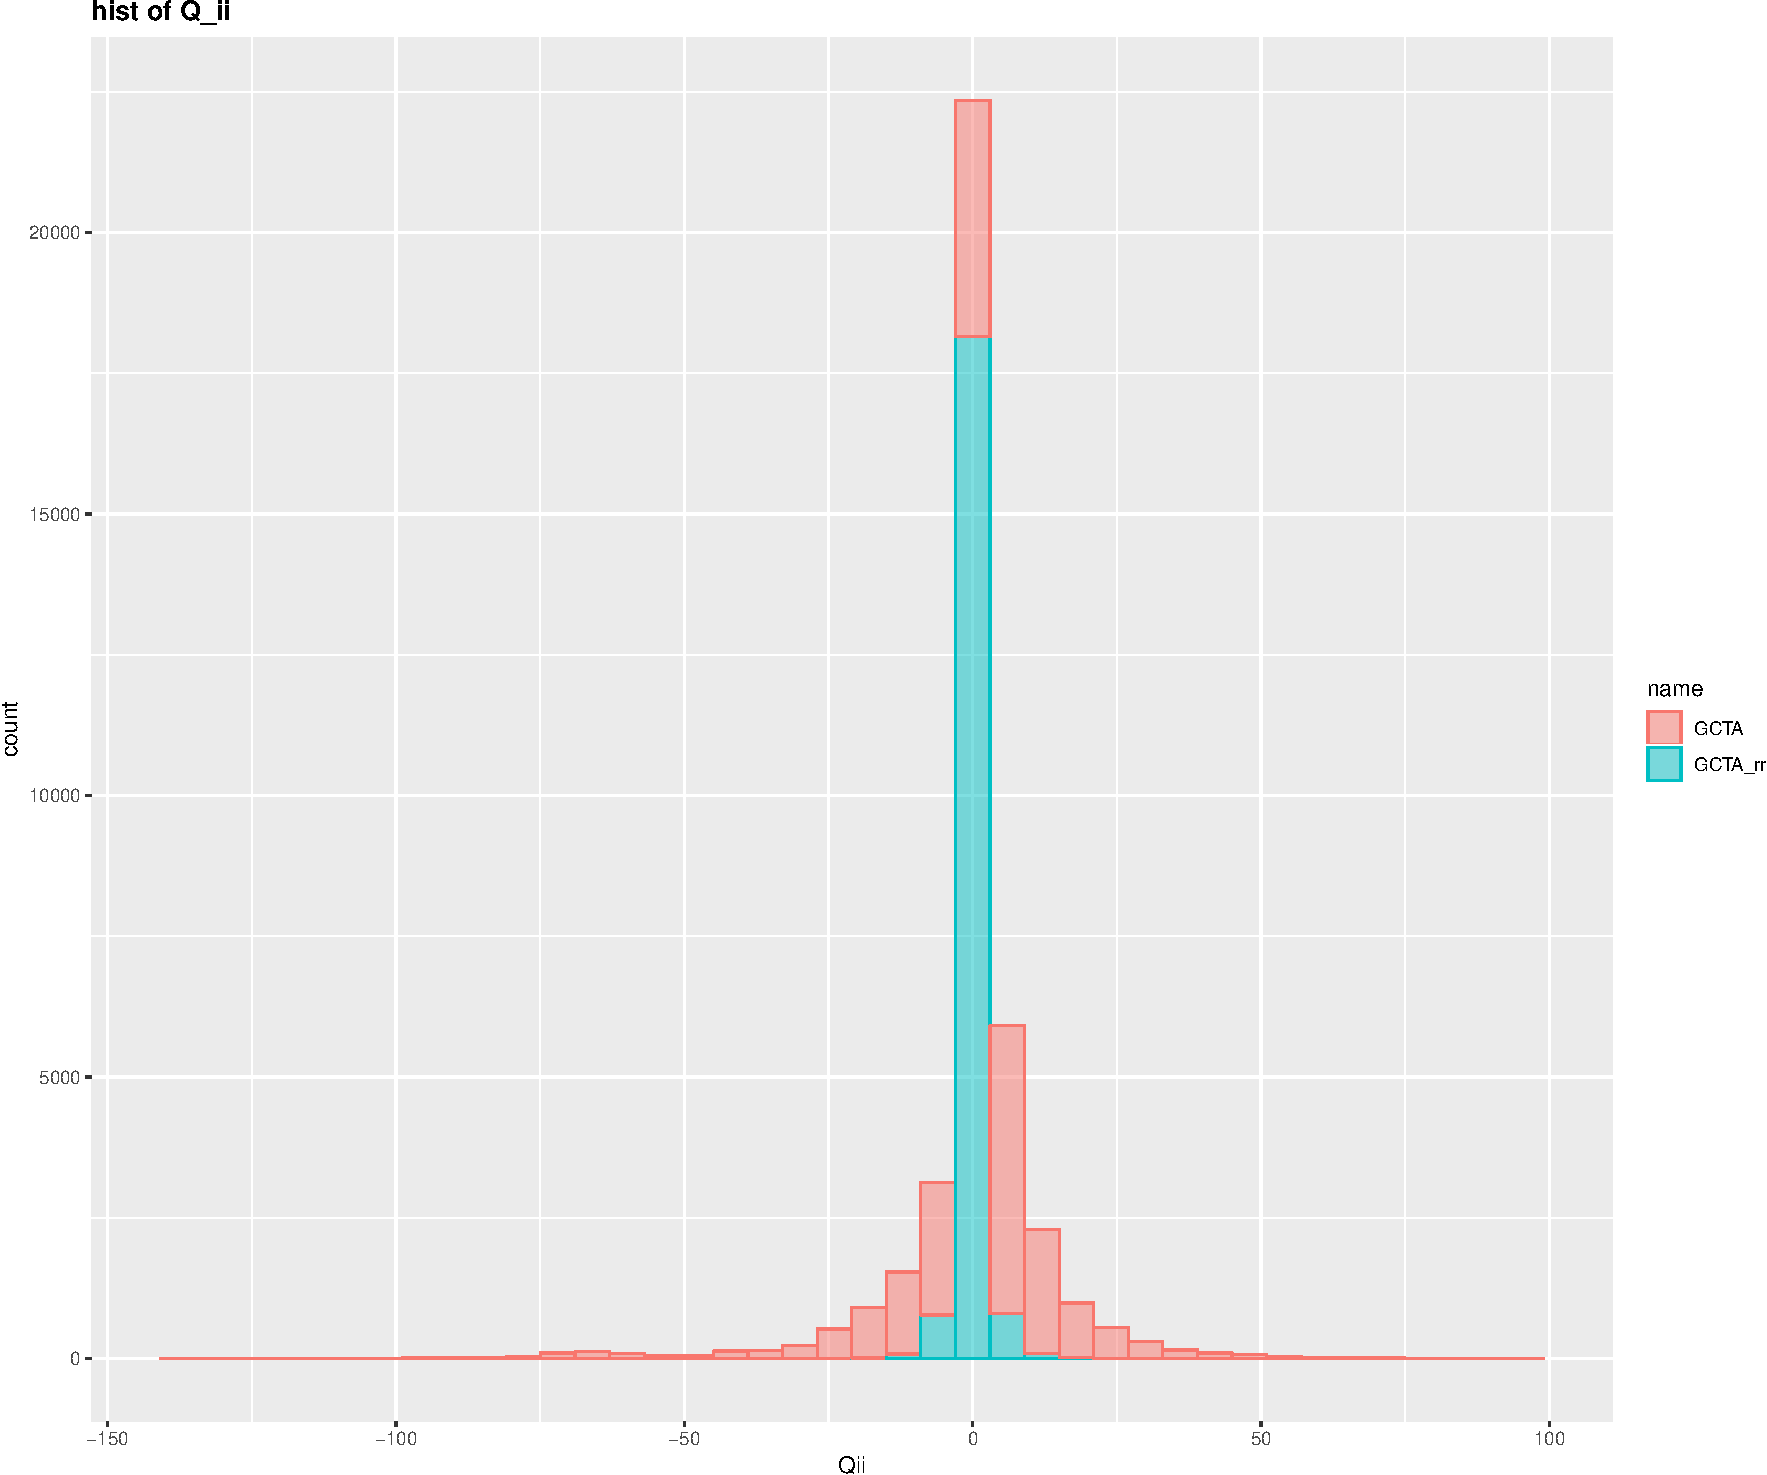
\includegraphics{GCTA_and_rr_v_jack_correction_files/figure-latex/unnamed-chunk-6-1.pdf}

\subsubsection{setup}\label{setup-1}

\begin{itemize}
\tightlist
\item
  Independent
\item
  Normal
\item
  \(p = 100\)
\item
  \(n = \{50, 75,100, 150, 200\}\)
\item
  with interaction terms
\item
  main effect: \(Var(X^T\beta) = 0\) \newpage
\end{itemize}

\subsubsection{n = 50}\label{n-50-1}

\begin{verbatim}
        main_effect_GCTA   v_jack v_jack_corr
GCTA             0.0e+00 0.00e+00     0.0e+00
GCTA_rr          7.1e-07 2.44e-14     2.4e-14
\end{verbatim}

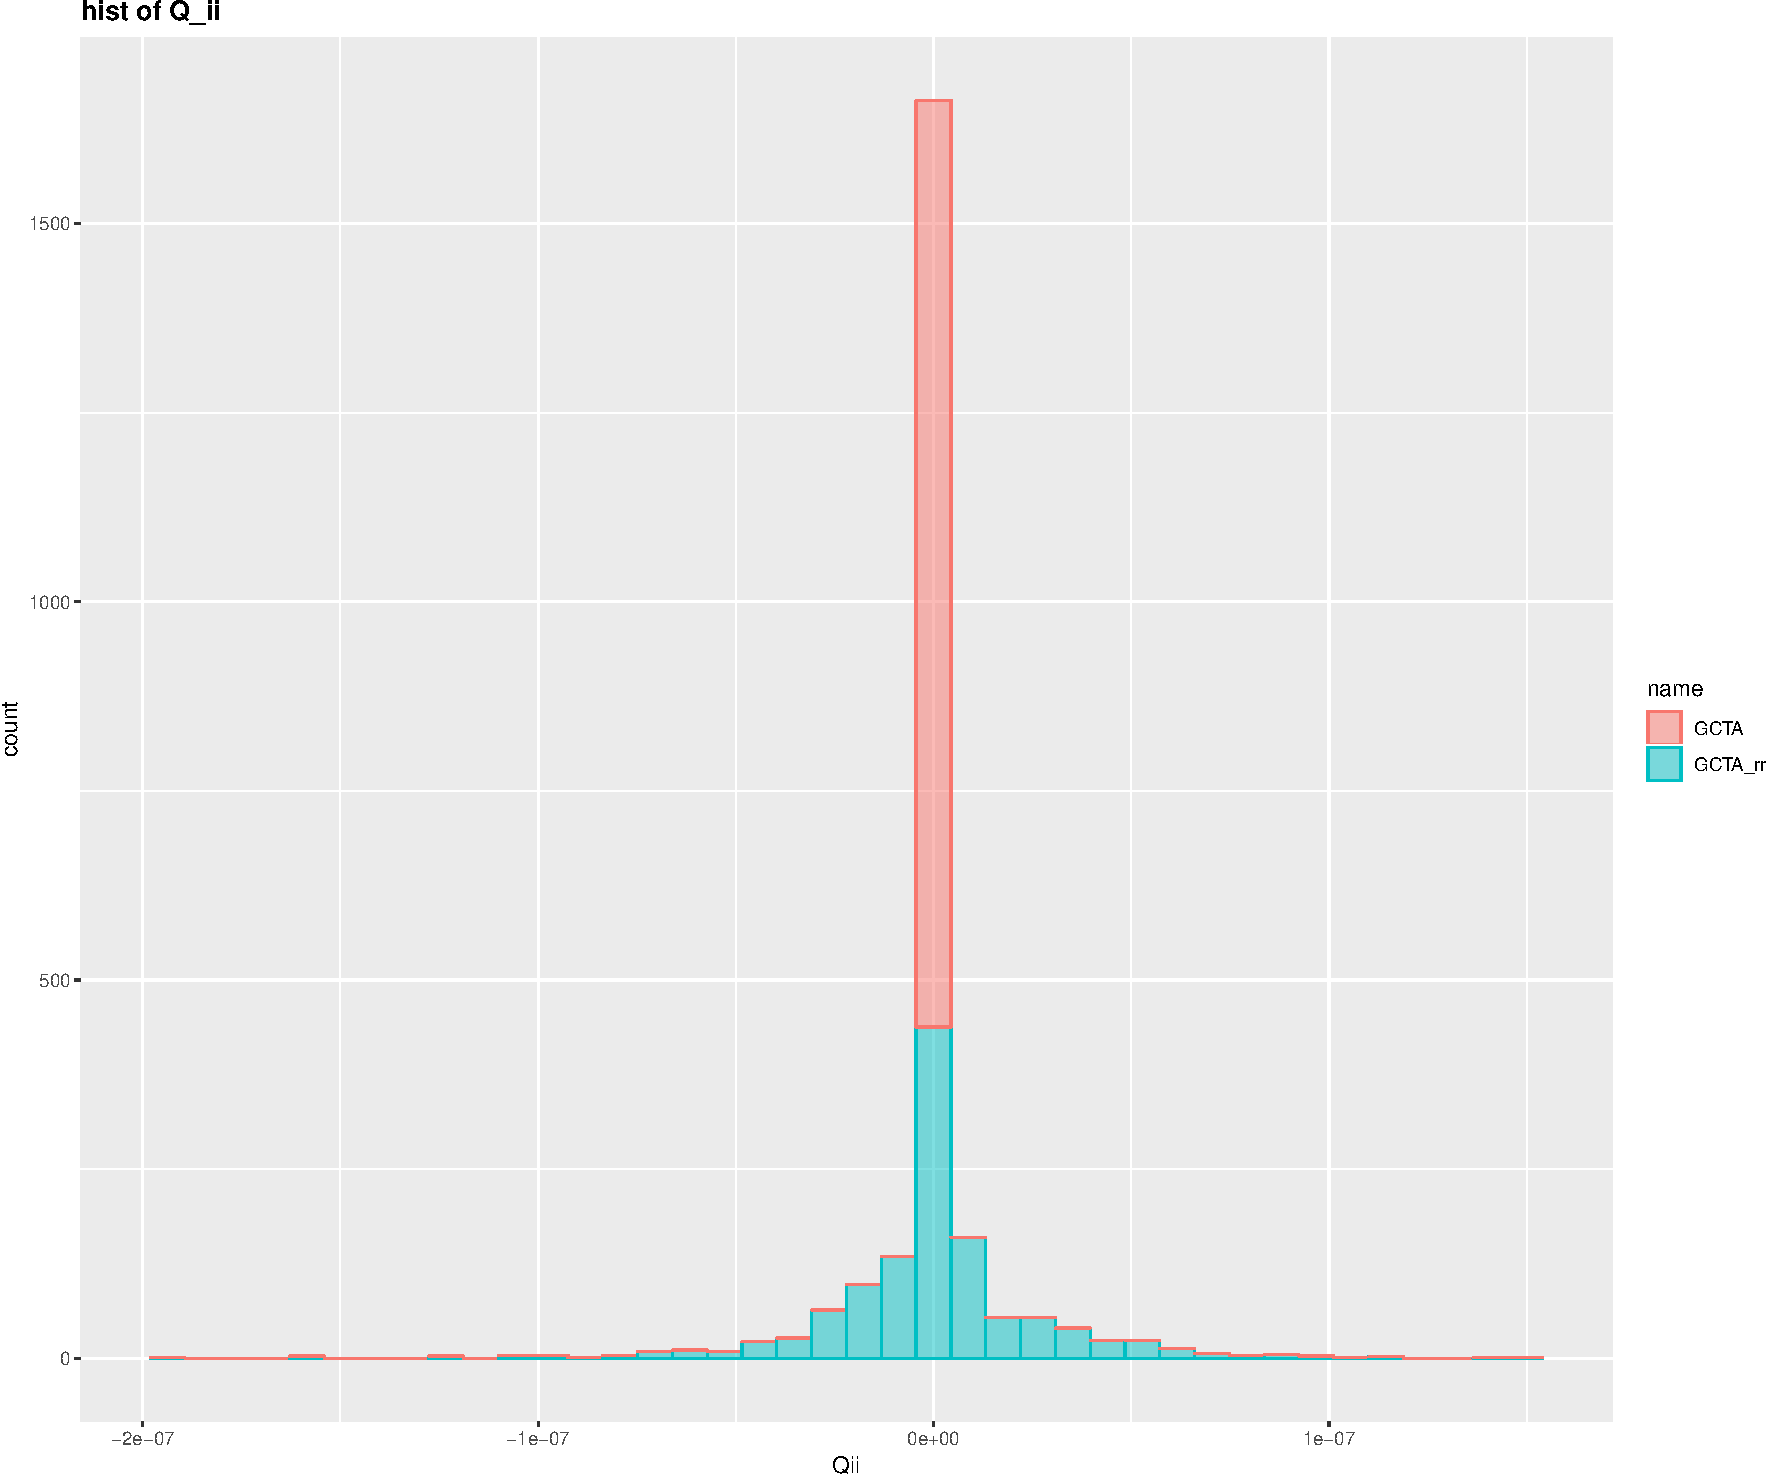
\includegraphics{GCTA_and_rr_v_jack_correction_files/figure-latex/unnamed-chunk-8-1.pdf}
\newpage

\subsubsection{n = 75}\label{n-75-1}

\begin{verbatim}
        main_effect_GCTA   v_jack v_jack_corr
GCTA             0.0e+00 0.00e+00    0.00e+00
GCTA_rr          9.5e-07 1.72e-14    1.69e-14
\end{verbatim}

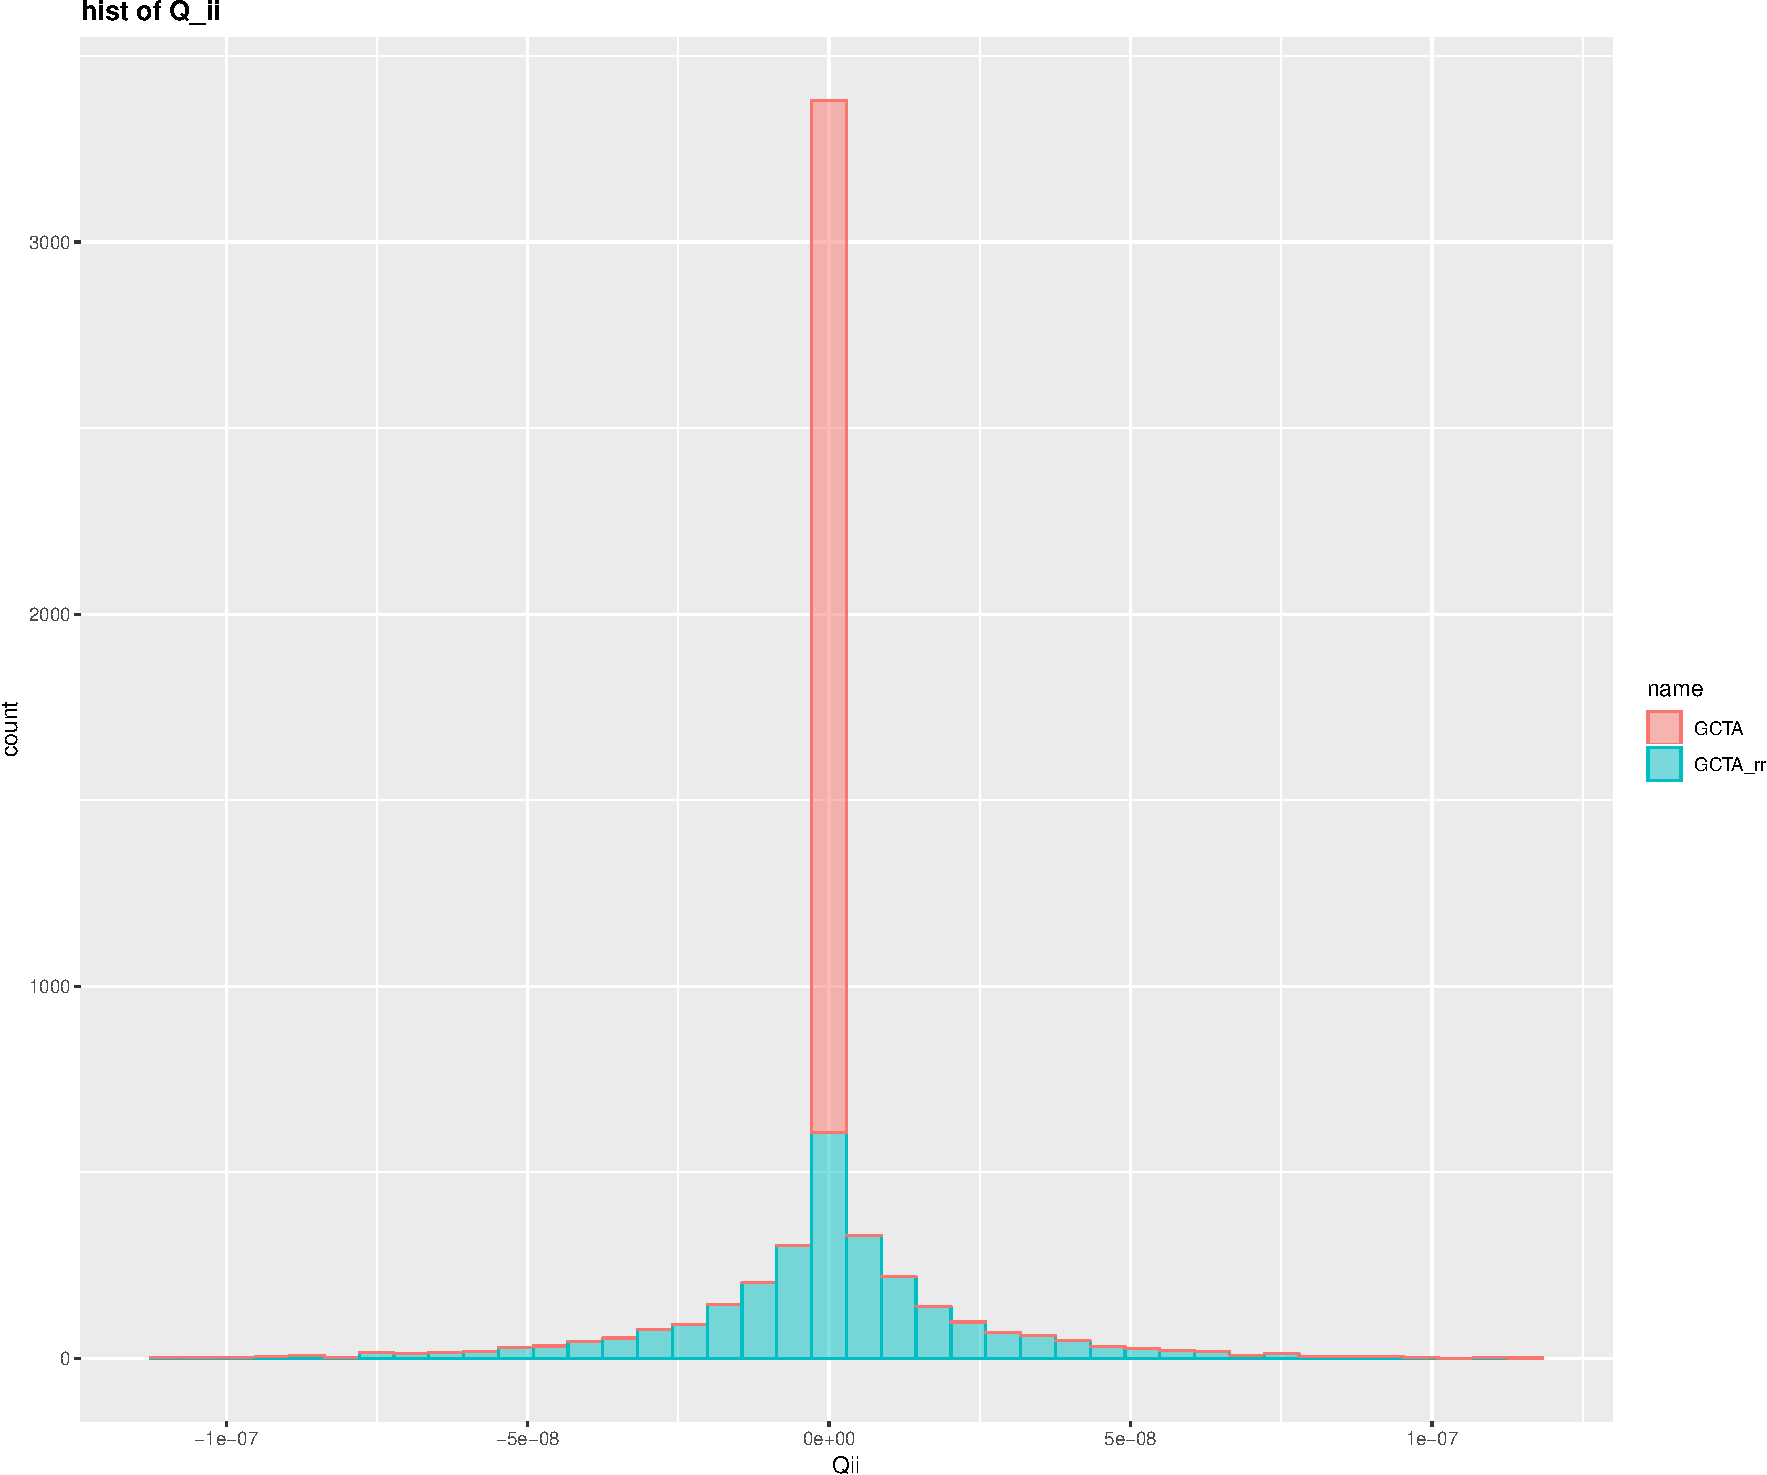
\includegraphics{GCTA_and_rr_v_jack_correction_files/figure-latex/unnamed-chunk-9-1.pdf}
\newpage

\subsubsection{n = 100}\label{n-100-1}

\begin{verbatim}
        main_effect_GCTA v_jack v_jack_corr
GCTA             0.0e+00 0.0104       -1.11
GCTA_rr          7.7e-07 0.0104       -1.11
\end{verbatim}

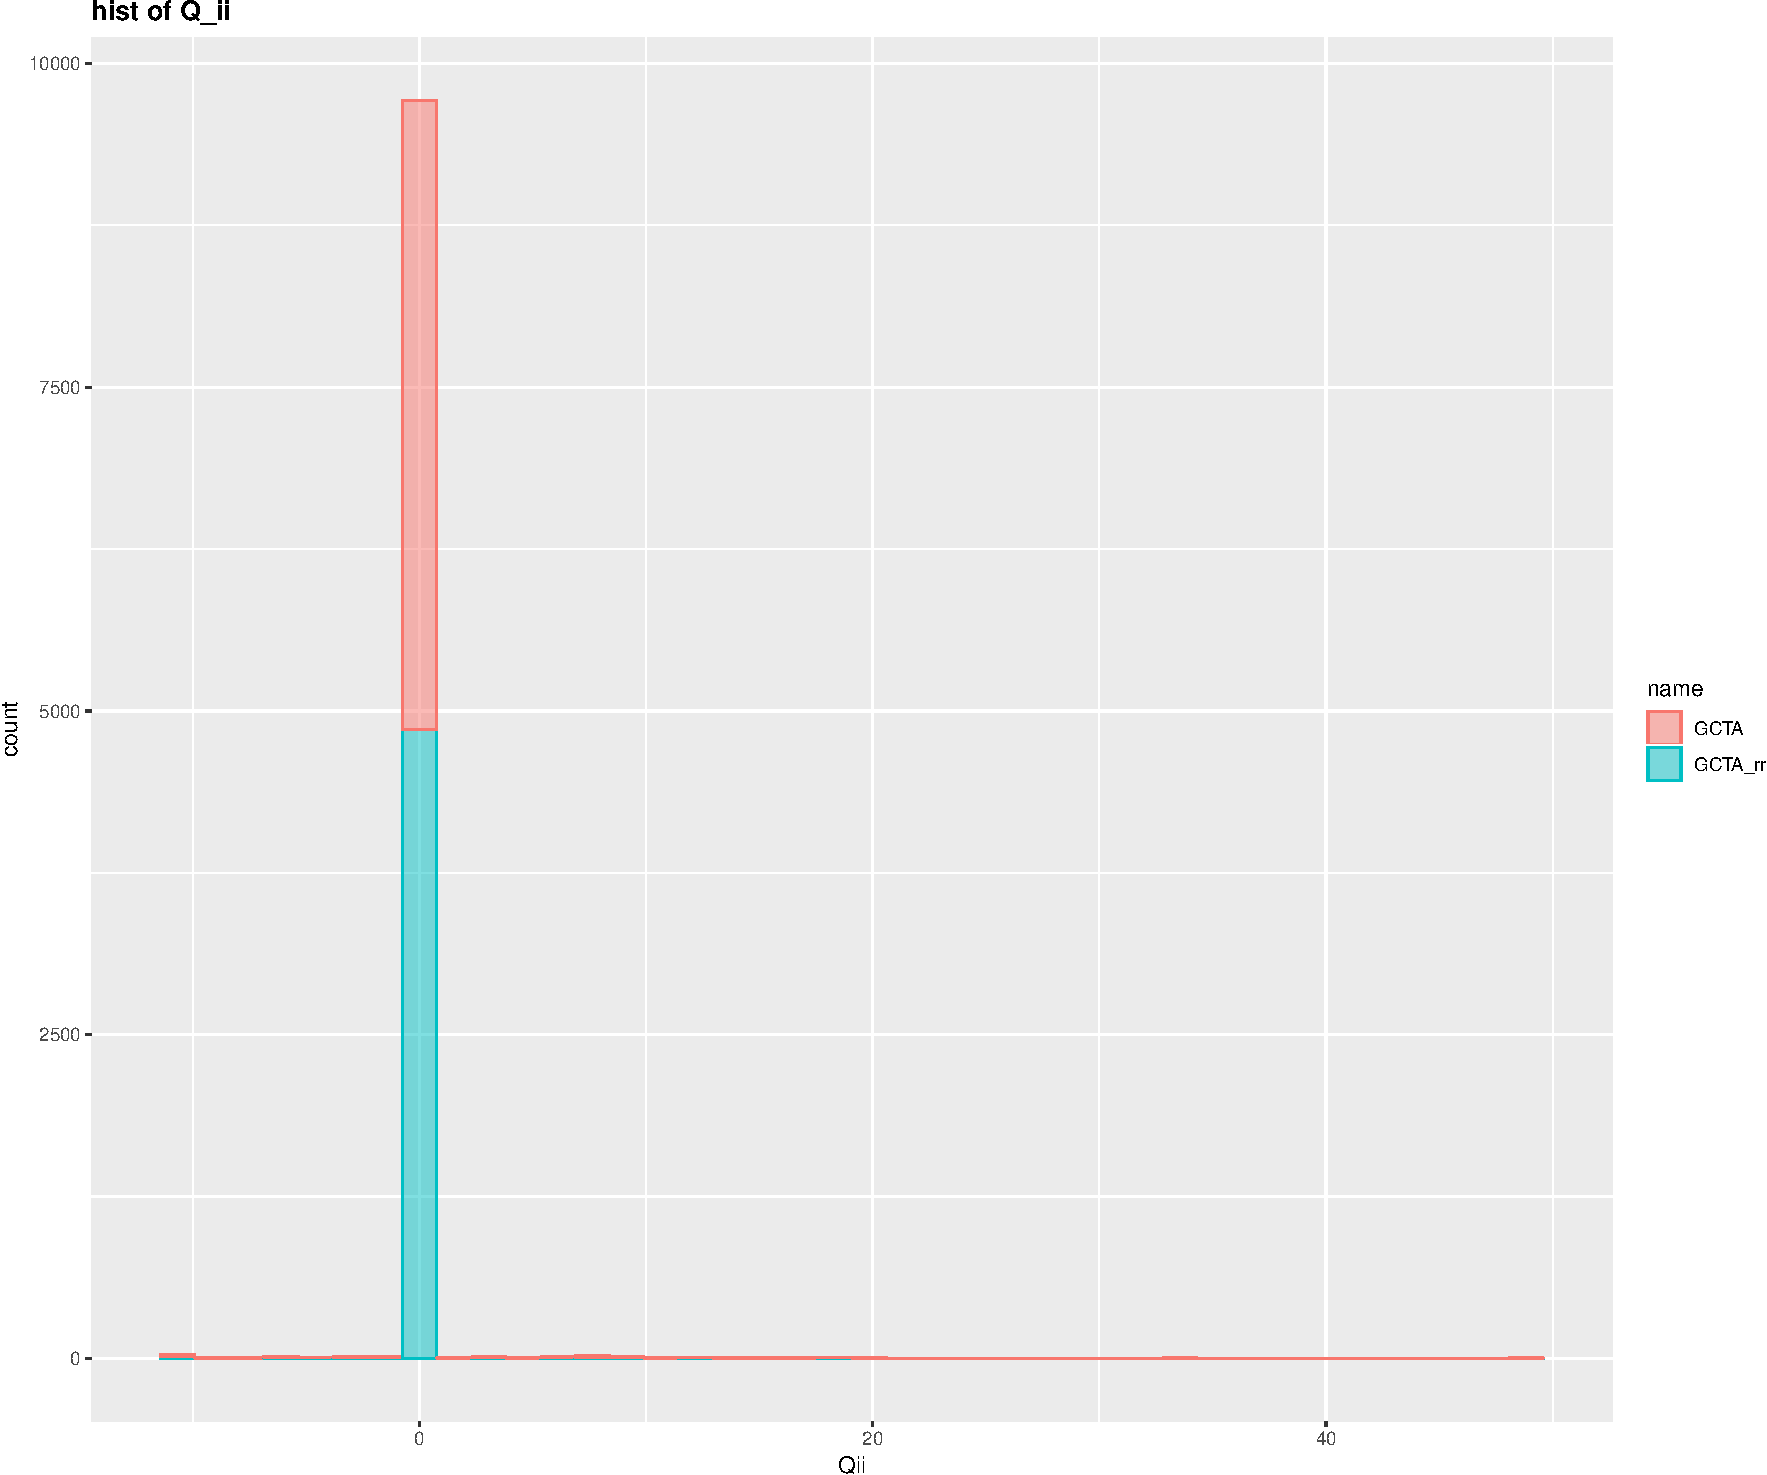
\includegraphics{GCTA_and_rr_v_jack_correction_files/figure-latex/unnamed-chunk-10-1.pdf}
\newpage

\subsubsection{n = 150}\label{n-150-1}

\begin{verbatim}
        main_effect_GCTA v_jack v_jack_corr
GCTA               0.595  1.305    -100.040
GCTA_rr            0.609  0.807       0.191
\end{verbatim}

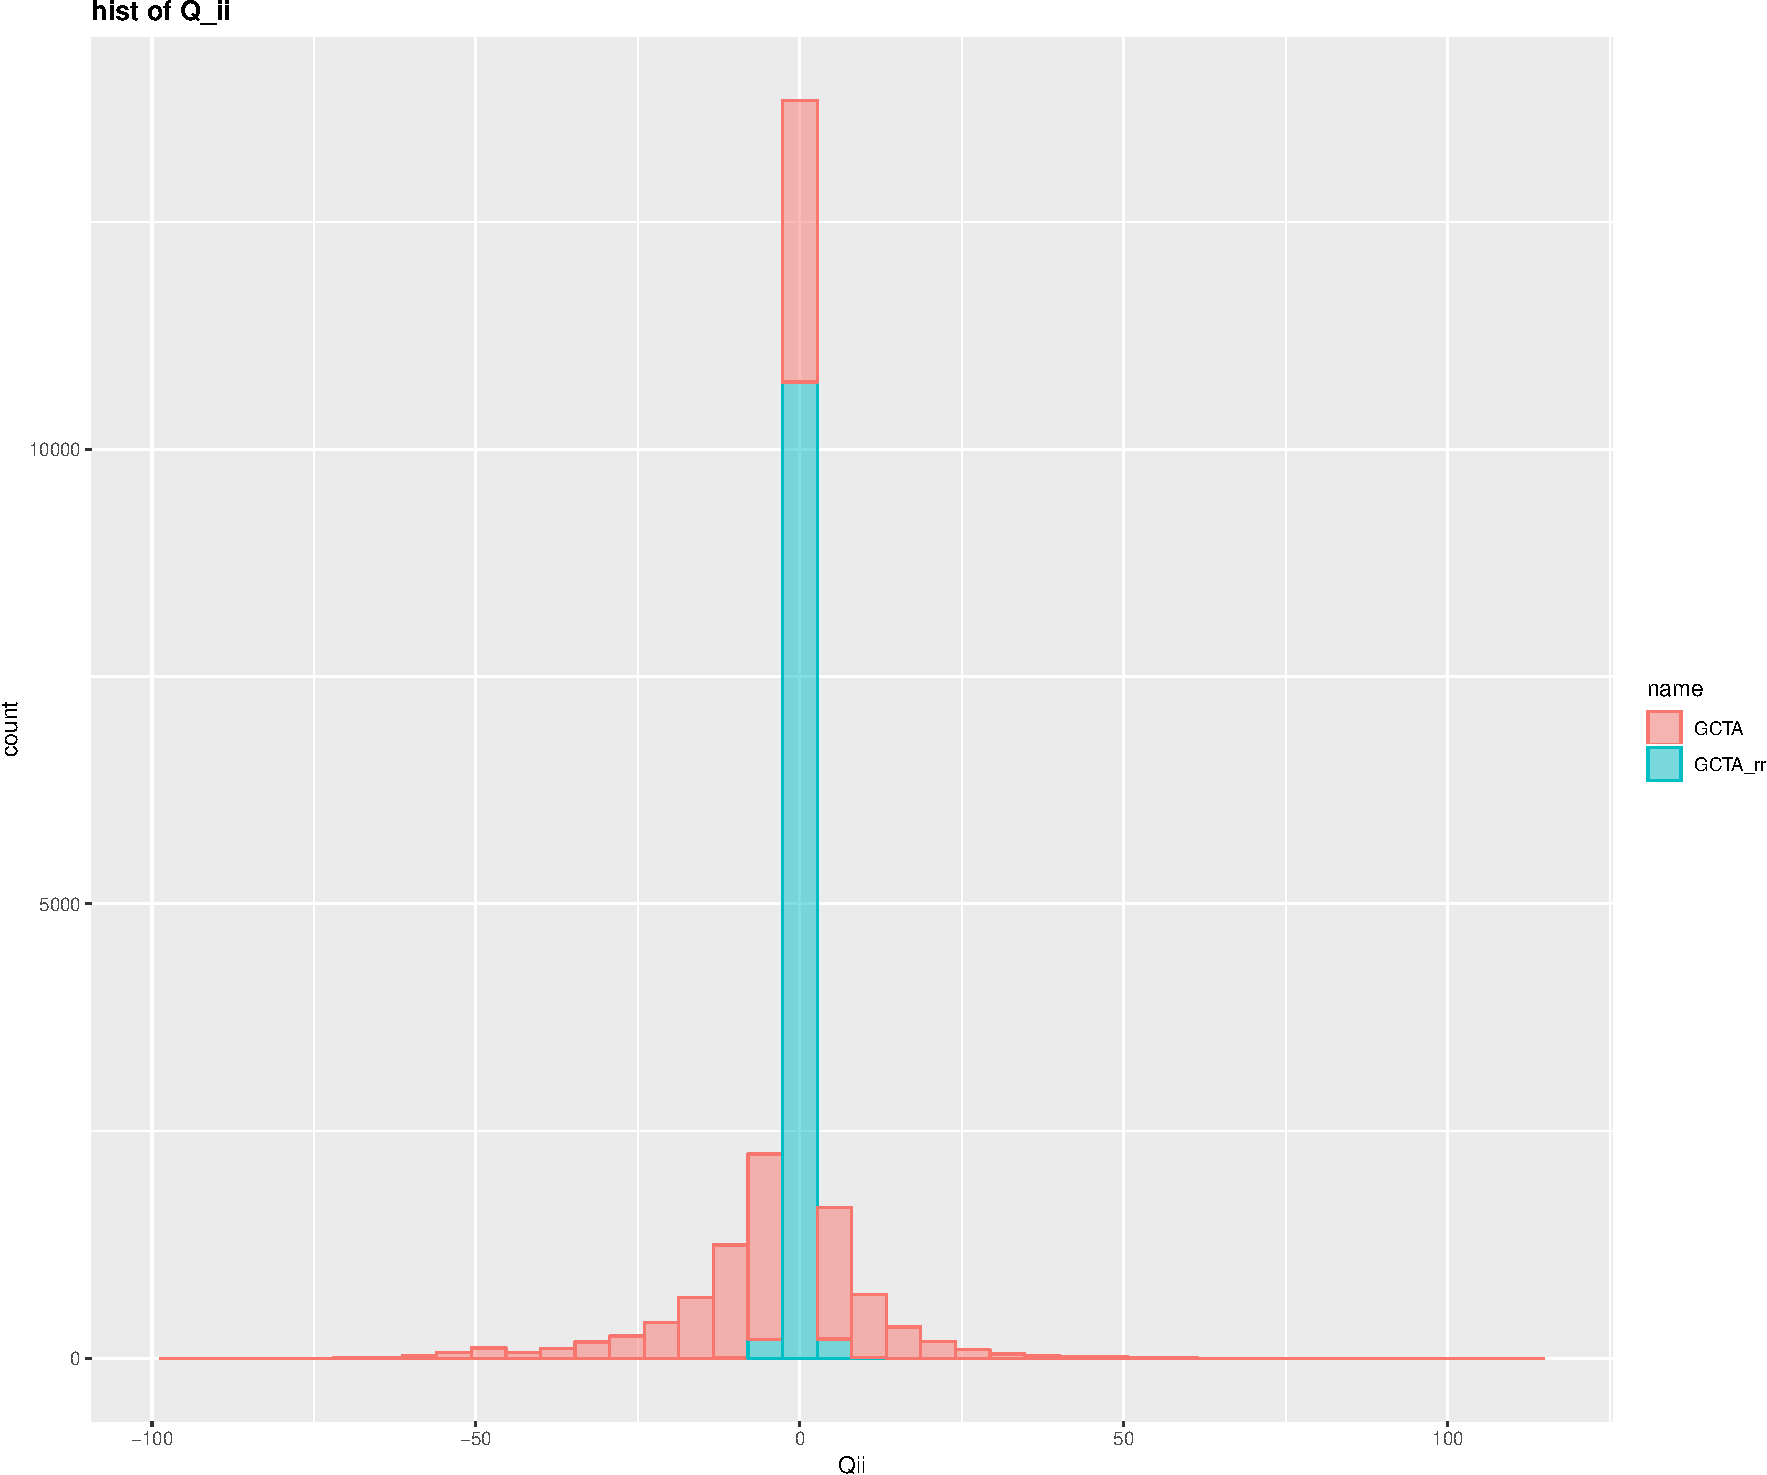
\includegraphics{GCTA_and_rr_v_jack_correction_files/figure-latex/unnamed-chunk-11-1.pdf}
\newpage

\subsubsection{n = 200}\label{n-200-1}

\begin{verbatim}
        main_effect_GCTA v_jack v_jack_corr
GCTA               0.106  0.696      -57.22
GCTA_rr            0.118  0.482       -0.95
\end{verbatim}

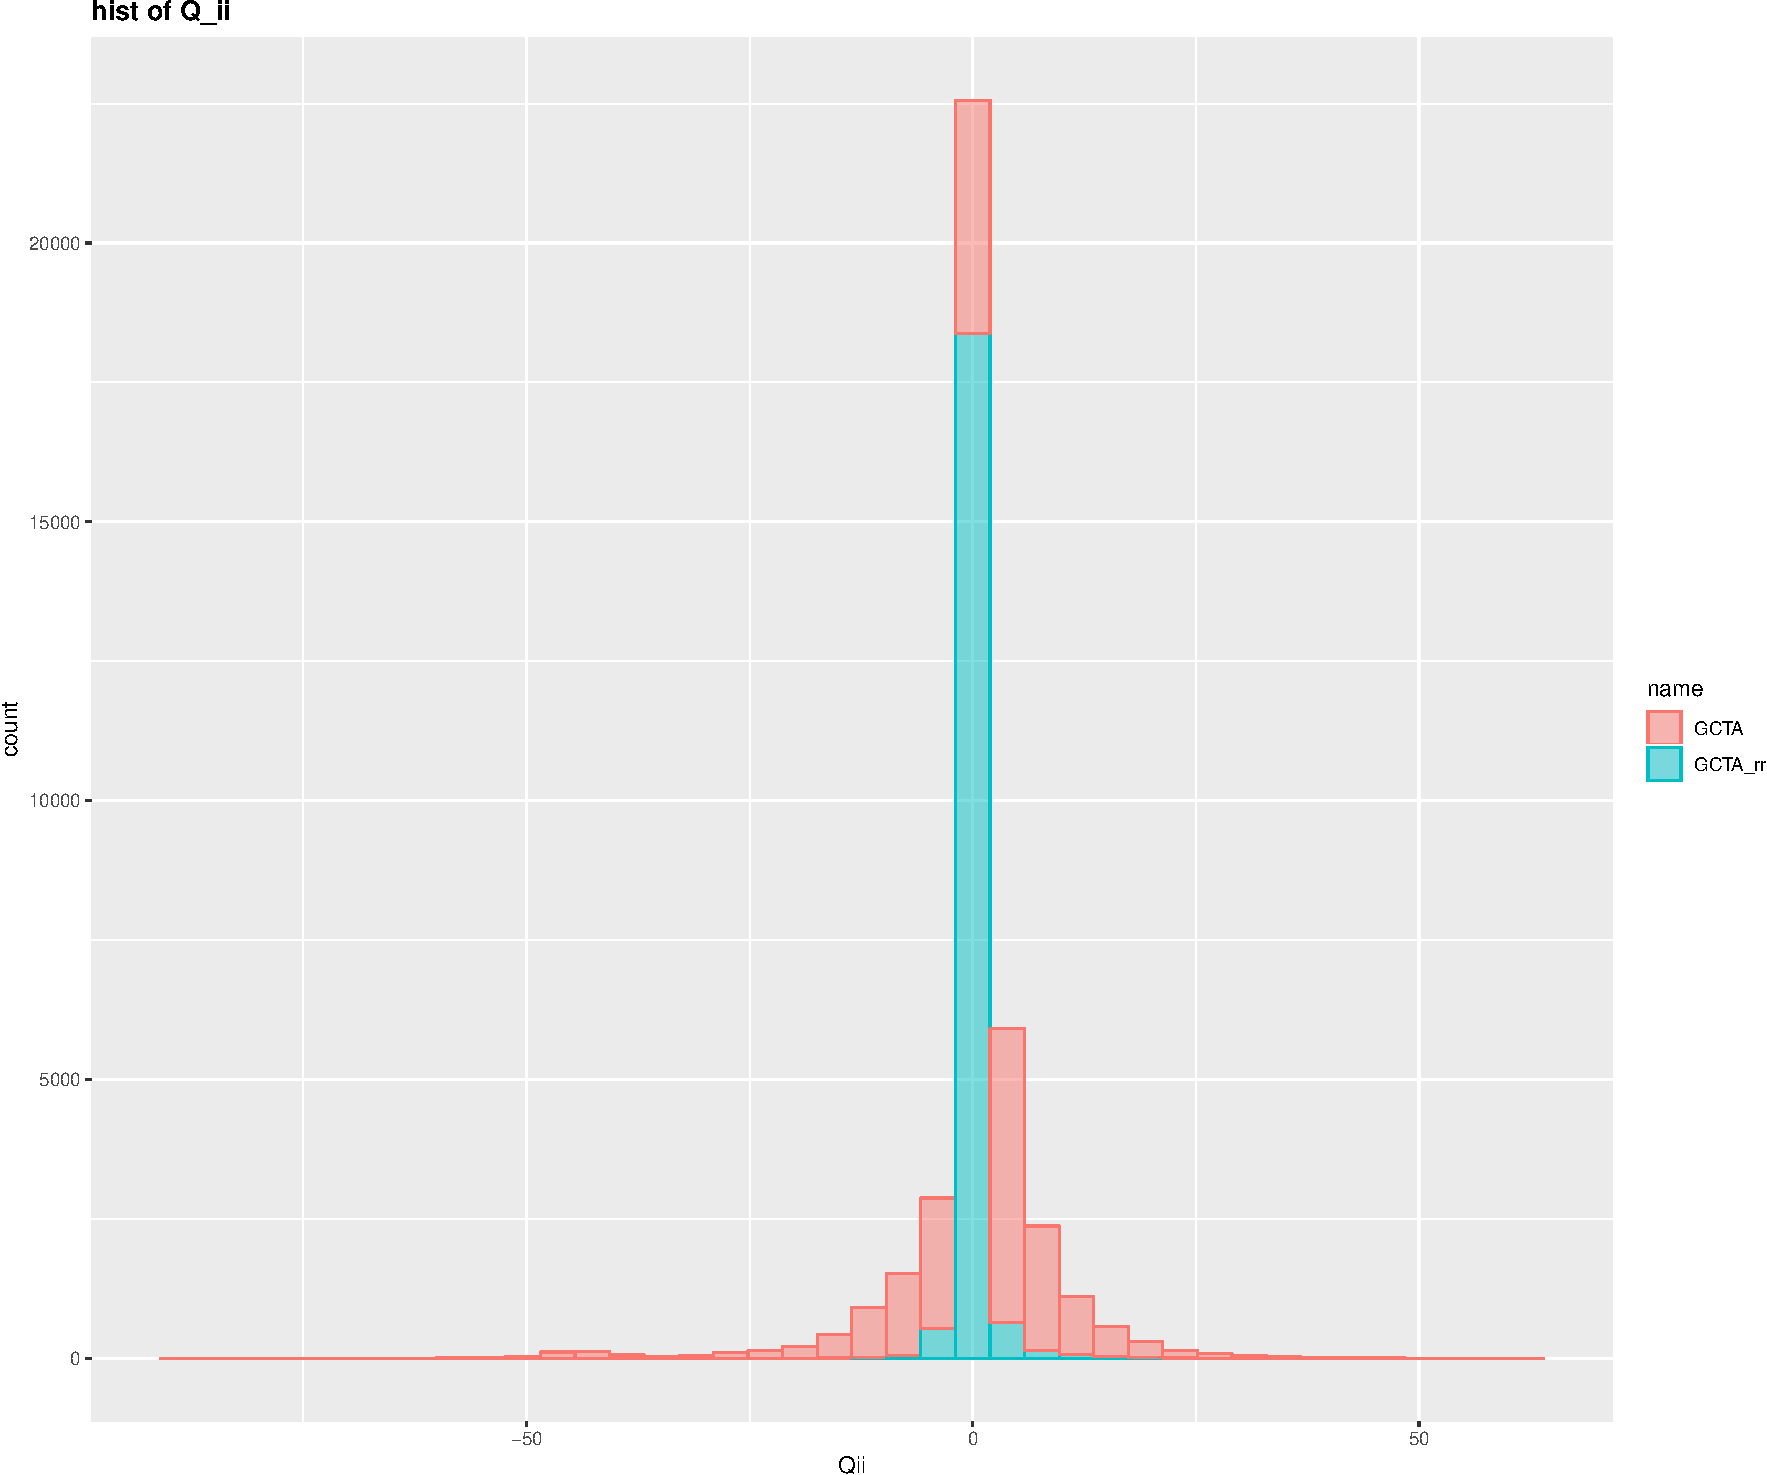
\includegraphics{GCTA_and_rr_v_jack_correction_files/figure-latex/unnamed-chunk-12-1.pdf}


\end{document}
